\documentclass{article}
\usepackage[catalan]{babel}
\usepackage[latin1]{inputenc}   % Permet usar tots els accents i car�ters llatins de forma directa.
\usepackage{enumerate}
\usepackage{amsfonts, amscd, amsmath, amssymb}
\usepackage{eepic}
\usepackage{graphicx}

%NOTA: si usam eepic hem de compilar a .dvi o .ps (NO PDF)

\setlength{\textwidth}{16cm}
\setlength{\textheight}{24cm}
\setlength{\oddsidemargin}{-0.3cm}
\setlength{\evensidemargin}{0.25cm} \addtolength{\headheight}{\baselineskip}
\addtolength{\topmargin}{-3cm}

\newcommand\Z{\mathbb{Z}}
\newcommand\R{\mathbb{R}}
\newcommand\N{\mathbb{N}}
\newcommand\Q{\mathbb{Q}}
\newcommand\K{\Bbbk}
\newcommand\C{\mathbb{C}}


\begin{document}

\begin{center}
\textbf{Problemes resolts Tema 3: processos estoc\`astics}
\end{center}

\vskip 0.5 cm
\noindent
\textbf{Problema 1.}
Considerem el proc\'es aleatori amb temps discret $X(n)$
definit a continuaci\'o. Es llan\c{c}a una moneda a l'aire i si surt
cara $X(n)=1$, en cas contrari $X(n)=-1$, per a tot $n$.

\begin{enumerate}[a)]
\item Dibuixau alguns camins de mostra del proc\'es.
\item Calculau la funci\'o de probabilitat de $X(n)$.
\item Calculau la funci\'o de probabilitat conjunta  de $X(n)$ i
$X(n+k)$.
\item Calculau $\mu_{X}(n)$ y $C_{X}(n,m)$.
\end{enumerate}


\vskip 0.3 cm
\noindent
\textbf{Soluci\'o:}

\vskip 0.2 cm
\noindent
\textbf{a)}

\vskip 0.2 cm
\begin{center}
\begin{tabular}{ccc}
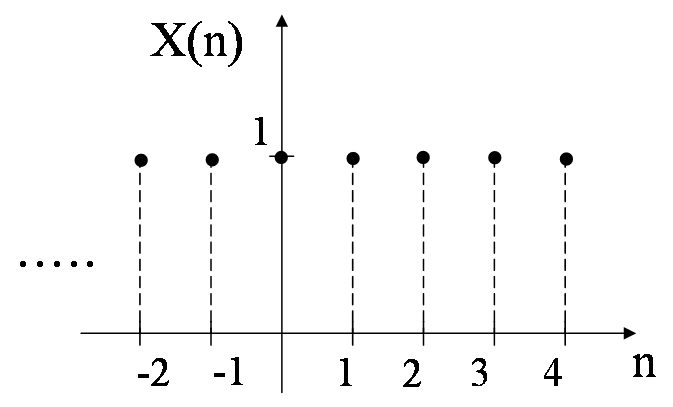
\includegraphics[width=5cm]{figprob1T3a.png}
&
$\qquad$
&
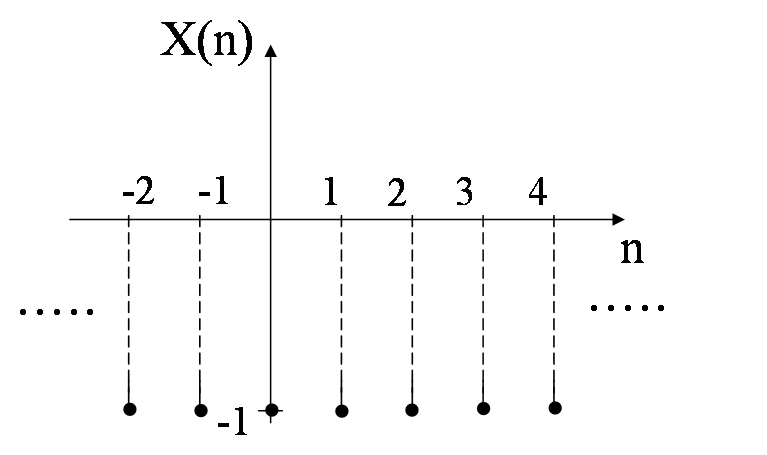
\includegraphics[width=5.5cm]{figprob1T3b.png} 
\\ \\
Realitzaci\'o del proc\'es quan la moneda surt cara 
& $\qquad$ &
Realitzaci\'o del proc\'es quan la moneda surt creu 
\end{tabular}
\end{center}


\vskip 0.2 cm
\noindent
\textbf{b)}
\[
P(X_n=x)=\begin{cases}
0  \qquad \text{si } x \notin \{ -1, 1 \} & \\
P(X_n=1)=P(\text{cara})=\frac{1}{2} & \\
P(X_n=-1)=P(\text{creu})=\frac{1}{2} & 
\end{cases}
\]

\vskip 0.2 cm
\noindent
\textbf{c)}
\[
P(X_n=x, X_{n+k}=y)=P(X_{n+k}=y | X_n=x) \cdot P(X_n=x)=\begin{cases}
0 \qquad \text{si } x \text{ \'o } y \notin \{ -1, 1 \} & \\
P(X_{n+k}=1 | X_n=-1) \cdot P(X_n=-1)= 0 \cdot \frac{1}{2}=0 & \\
P(X_{n+k}=-1 | X_n=1) \cdot P(X_n=1)= 0 \cdot \frac{1}{2}=0 & \\
P(X_{n+k}=1 | X_n=1) \cdot P(X_n=1)= 1 \cdot \frac{1}{2}=\frac{1}{2} & \\
P(X_{n+k}=-1 | X_n=-1) \cdot P(X_n=1)= -1 \cdot \frac{1}{2}=\frac{1}{2} 
\end{cases}
\]

\vskip 0.2 cm
\noindent
\textbf{d)}
\[
\begin{array}{l}
\mu_X(n)=E(X_n)=1 \cdot P(X_n=1) + (-1) \cdot P(X_n=-1) = \frac{1}{2} - \frac{1}{2}=0 \\ \\
R_X(n, m)=E(X_n \cdot X_{n+m})=
\begin{cases} 
\text{si } m=n & \\
& E(X_n^2)=1^2 \cdot P(X_n=1)+(-1)^2 \cdot P(X_n=-1)=\frac{1}{2} + \frac{1}{2}=1 \\
\text{si } m \neq n & \\ 
&
\begin{array}{ll}
E(X_n \cdot X_{n+m})= & 1 \cdot 1 \cdot P(X_n=1, X_{n+m}=1) + \\
                      & 1 \cdot (-1) \cdot P(X_n=1, X_{n+m}=-1)+ \\
                      &  (-1) \cdot 1 \cdot P(X_n=-1, X_{n+m}=1) + \\
                      & (-1) \cdot (-1) \cdot P(X_n=-1, X_{n+m}=-1)= \\
                      & = \frac{1}{2} + 0 + 0+ \frac{1}{2}=1
\end{array}
\end{cases}
\\ \\
C_X(n, m)=R_X(n, m)-\mu_X(n) \cdot \mu_X(n+m)=1 - 0 \cdot 0 = 1
\end{array}
\]

\newpage

\noindent
\textbf{Problema 2.}
Considerem el proc\'es aleatori en temps  discret $X(n)$
definit a continuaci\'o. Es llan\c{c}a una moneda a l'aire;  si surt
cara $X(n)=(-1)^n$ i $X(n)=(-1)^{n+1}$ si surt creu, per a tot $n$.

\begin{enumerate}[a)]
\item Dibuixau alguns camins de mostra del proc\'es.
\item Calculau la funci\'o de probabilitat de $X(n)$.
\item Calculau la funci\'o de probabilitat conjunta  de $X(n)$ i
$X(n+k)$.
\item Calculau $\mu_{X}(n)$ y $C_{X}(n,m)$.
\end{enumerate}

\vskip 0.3 cm
\noindent
\textbf{Soluci\'o:}


\vskip 0.2 cm
\noindent
\textbf{a)}

\vskip 0.2 cm
\begin{center}
\begin{tabular}{ccc}
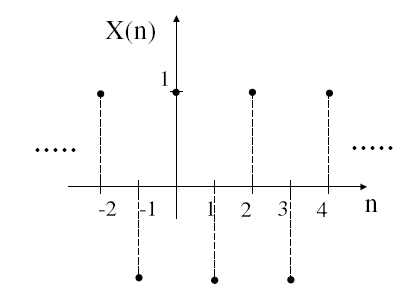
\includegraphics[width=5cm]{figprob2T3a.png}
&
$\qquad$
&
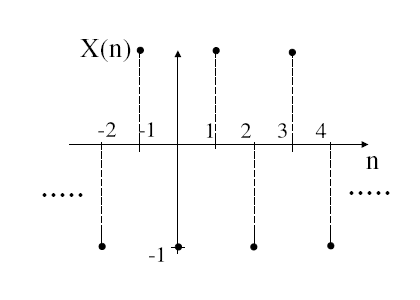
\includegraphics[width=5.5cm]{figprob2T3b.png} 
\\ \\
Realitzaci\'o del proc\'es quan la moneda surt cara 
& $\qquad$ &
Realitzaci\'o del proc\'es quan la moneda surt creu 
\end{tabular}
\end{center}


\vskip 0.2 cm
\noindent
\textbf{b)}

\[
\begin{array}{l}
P(X(n) = x) = 0 \qquad \text{si } x \notin \{-1, +1\} 
\\ \\
P(X(n) = 1) = \begin{cases} \text{si $n$ parell} & P(cara)=1/2 \\
\text{si $n$ imparell} & P(creu)=1/2 \end{cases}
\\ \\
P(X(n) = -1) = \begin{cases} \text{si $n$ parell} & P(creu)=1/2 \\
\text{si $n$ imparell} & P(cara)=1/2 \end{cases}
\end{array}
\]

\noindent
En resum:
\[
P(X(n)=x)=\begin{cases} 0 & \text{si } x \notin \{-1, +1\} \\ \\
\frac{1}{2} & \text{si } x = 1 \quad \text{ o } \quad x=-1
\end{cases}
\]

\vskip 0.2 cm
\noindent
\textbf{c)}
\[
\begin{array}{l}
P(X(n) = x, X(n+k)=y) = 0 \qquad \text{si } x, y \notin \{-1, +1\}  \\ \\
\text{si } k= 0 \quad \text{:}\\
P(X(n) = x, X(n)=y) = \begin{cases} 0 & \text{si } x \neq y \\ P(X(n) = x)=1/2 & \text{si } x=y \quad \text{ i } x \in \{-1, +1\} \end{cases}\\ \\
\text{si $k$ parell} \quad \text{:}\\
P(X(n) = 1, X(n+k)=-1) = 0 \\ \\
P(X(n) = -1, X(n+k)=1) = 0 \\ \\
P(X(n) = 1, X(n+k)=1) = P(X(n)=1)=1/2 \\ \\
P(X(n) = -1, X(n+k)=-1) = P(X(n)=-1)=1/2 \\ \\
\text{si $k$ imparell} \quad \text{:}\\
P(X(n) = -1, X(n+k)=-1) = 0 \\ \\
P(X(n) = 1, X(n+k)=1) = 0 \\ \\
P(X(n) = 1, X(n+k)=-1) = P(X(n)=1)=1/2 \\ \\
P(X(n) = -1, X(n+k)=1) = P(X(n)=-1)=1/2 
\end{array}
\]

\vskip 0.2 cm
\noindent
\textbf{d)}
\[
\begin{array}{l}
\mu_X(n)=E(X(n))=1 \cdot P(X(n) = 1) + (-1) \cdot P(X(n)=-1) = 1 \cdot \frac{1}{2} - 1 \cdot \frac{1}{2} = 0  \\ \\
R_X(n, m)=E(X(n) \cdot X(m))= \\ \\
=\begin{cases} \text{si } n=m &  E(X(n) \cdot X(n))= E((X(n)^2)=E(1)=1 \\ \\
\text{ si $|m-n|$ parell} & 
\begin{array}{ll} E(X(n) \cdot X(m))=& 1 \cdot 1 \cdot P(X(n)=1, X(m)=1) + \\
& + 1 \cdot (-1) \cdot P(X(n)=1, X(m)=-1)+\\
&(-1) \cdot 1 \cdot P(X(n)=-1, X(m)=1) +\\ 
&(-1) \cdot (-1) \cdot P(X(n)=-1, X(m)=-1)=\frac{1}{2}-0-0+\frac{1}{2}=1 \end{array}\\ \\
\text{ si $|m-n|$ imparell} & 
\begin{array}{ll} E(X(n) \cdot X(m))=& 1 \cdot 1 \cdot P(X(n)=1, X(m)=1) + \\
& + 1 \cdot (-1) \cdot P(X(n)=1, X(m)=-1)+\\
&(-1) \cdot 1 \cdot P(X(n)=-1, X(m)=1) +\\ 
&(-1) \cdot (-1) \cdot P(X(n)=-1, X(m)=-1)=0-\frac{1}{2}-\frac{1}{2}+0=-1  \end{array}
\end{cases}
\\ \\ \\ \\
C_X(n, m)=R_X(n, m)-\mu_X(n) \cdot \mu_X(m) = R_X(n, m)-0 \cdot 0 = 
\begin{cases} 1 & \text{si $|n-m|$ parell o 0} \\ \\ -1 & \text{si $|n-m|$ imparell} \end{cases}
\end{array}
\]




\newpage

\noindent
\textbf{Problema 3.}
Sigui $g(t)$ un pols rectangular a l'interval $(0,1)$, \'es a
dir $g(t)=1$ si $t\in(0,1)$ i zero a la resta de casos. Considerem
el proc\'es aleatori definit per $X(t)=Ag(t)$ on $A=\pm 1$ amb la
mateixa probabilitat.

\begin{enumerate}[a)]
\item Calculau la funci\'o de probabilitat de $X(t)$.
\item Calculau $\mu_{X}(t)$
\item Calculau la funci\'o de probabilitat conjunta  de $X(t)$ i
$X(t+d)$, amb $d > 0$.
\item Calculau  $C_{X}(t,t+d)$ amb $d>0$.
\end{enumerate}

\vskip 0.3 cm
\noindent
\textbf{Soluci\'o:}

\vskip 0.2 cm
\noindent
\textbf{a)} 

\vskip 0.2 cm
\begin{center}
\begin{tabular}{ccc}
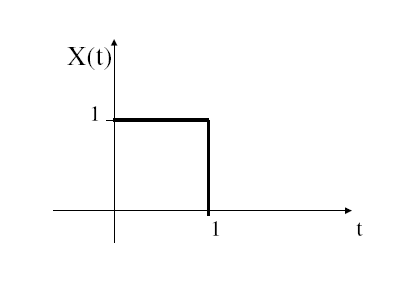
\includegraphics[width=5cm]{figprob3T3a.png}
&
$\qquad$
&
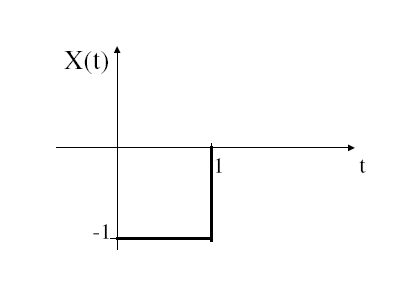
\includegraphics[width=5.5cm]{figprob3T3b.png} 
\end{tabular}

Les dues possibles realitzacions del proc\'es
\end{center}
 
\[
\begin{array}{l}
P(X(t) = x) = 0 \qquad \text{ si } x \notin \{-1, 0, 1 \} \\ \\
P(X(t) = 1)=P(Ag(t) = 1)=\begin{cases} \text{si } t \notin (0, 1) & 0 \\ \\ \text{si } t \in (0, 1) & P(A=1)=1/2 \end{cases} \\ \\
P(X(t) = -1)=P(Ag(t) = -1)=\begin{cases} \text{si } t \notin (0, 1) & 0 \\ \\ \text{si } t \in (0, 1) & P(A=-1)=1/2 \end{cases} \\ \\
P(X(t) = 0)=P(Ag(t) = 0)=\begin{cases} \text{si } t \notin (0, 1) & 1 \\ \\ \text{si } t \in (0, 1) & P(A=0)=0 \end{cases} 
\end{array}
\]

\vskip 0.2 cm
\noindent
\textbf{b)} 
\[
\begin{array}{ll}
\mu_X(t)=E(X(t))=(-1) \cdot P(X(t)=-1) + 0 \cdot P(X(t)=0) + 1 \cdot P(X(t)=1) = 
\begin{cases} \text{si } t \notin (0, 1) & (-1) \cdot 0 + 0 \cdot 1 + 1 \cdot 0=0  
\\ \\ \text{si } t \in (0, 1) & 0 \cdot 0 + 1 \cdot \frac{1}{2} - 1 \cdot \frac{1}{2}=0 \end{cases} 
\end{array}
\]

\noindent
Per tant, $\mu_X(t)=0$ $\forall t$.

\newpage
\vskip 0.2 cm
\noindent
\textbf{c)} 

\[
\begin{array}{l}
P(X(t)=x, X(t+d)=y)=0 \qquad \text{si } x, y \notin \{-1, 0, 1\} \\ \\
\text{si } t \notin (0, 1) \quad \text{ i } \quad t+d \notin (0, 1) \text{ : }\\
P(X(t)=x, X(t+d)=y)=0 \qquad \text{si } x \neq 0 \quad \text{ o } \quad y \neq 0 \\ \\
P(X(t)=0, X(t+d)=0)=1 \\ \\
\text{si } t \in (0, 1) \quad \text{ i } \quad t+d \notin (0, 1) \text{ : }\\
P(X(t)=x, X(t+d)=y)=0 \qquad \text{si } x = 0 \quad \text{ o } \quad y \neq 0 \\ \\
P(X(t)=1, X(t+d)=0)=P(X(t)=1)=1/2 \\ \\
P(X(t)=-1, X(t+d)=0)=P(X(t)=-1)=1/2 \\ \\
\text{si } t \notin (0, 1) \quad \text{ i } \quad t+d \in (0, 1) \text{ : }\\
P(X(t)=x, X(t+d)=y)=0 \qquad \text{si } x \neq 0 \quad \text{ o } \quad y=0 \\ \\
P(X(t)=0, X(t+d)=1)=P(X(t+d)=1)=1/2 \\ \\
P(X(t)=0, X(t+d)=-1)=P(X(t+d)=-1)=1/2 \\ \\
\text{si } t \in (0, 1) \quad \text{ i } \quad t+d \in (0, 1) \text{ : }\\
P(X(t)=x, X(t+d)=y)=0 \qquad \text{si } x=0 \quad \text{ o } \quad y=0 \\ \\
P(X(t)=1, X(t+d)=-1)=0 \\ \\
P(X(t)=-1, X(t+d)=1)=0 \\ \\
P(X(t)=1, X(t+d)=1)=P(X(t)=1)=1/2 \\ \\
P(X(t)=-1, X(t+d)=-1)=P(X(t)=-1)=1/2 
\end{array}
\]


\vskip 0.2 cm
\noindent
\textbf{d)} 

\[
\begin{array}{ll}
C_X(t, t+d)&=R_X(t, t+d)-\mu(t) \mu(t+d) = R_X(t, t+d)-0 \cdot 0 = R_X(t, t+d) = E(X(t) \cdot X(t+d))= \\ \\
& = 0 \cdot 0 \cdot P(X(t)=0, X(t+d)=0) + 0 \cdot 1 \cdot P(X(t)=0, X(t+d)=1) + \\ \\
& + 0 \cdot (-1) \cdot P(X(t)=0, X(t+d)=-1) + 1 \cdot 0 \cdot P(X(t)=1, X(t+d)=0) + \\ \\
& + 1 \cdot 1 \cdot P(X(t)=1, X(t+d)=1) + 1 \cdot (-1) \cdot P(X(t)=1, X(t+d)=-1) + \\ \\
& + (-1) \cdot 0 \cdot P(X(t)=-1, X(t+d)=0) + (-1) \cdot 1 \cdot P(X(t)=-1, X(t+d)=1) + \\ \\
& + (-1) \cdot (-1) \cdot P(X(t)=-1, X(t+d)=-1) = \\ \\
& = P(X(t)=1, X(t+d)=1) - P(X(t)=1, X(t+d)=-1)- \\ \\
& - P(X(t)=-1, X(t+d)=1) + P(X(t)=-1, X(t+d)=-1) = \\ \\
& = \begin{cases} \text{si } t \in (0, 1) \quad \text{ i } \quad t+d \in (0, 1) & \frac{1}{2}-0+0+\frac{1}{2}=1 \\ \\
\text{en cas contrari } & 0-0-0+0=0 \end{cases}
\end{array}
\]

\newpage
\noindent
\textbf{Problema 4.}
 Un proc\'es aleatori est\`a definit per l'equaci\'o $Y(t)=g(t-T)$
on $g(t)$ \'es el pols del problema anterior 
($g(t)=1$ si $t\in(0,1)$ i zero sin\'o)
i $T$ \'es una v.a. amb
distribuci\'o uniforme a l'interval unitat.
\begin{enumerate}[a)]
\item Calculau la funci\'o de probabilitat de $Y(t)$.
\item Trobau la funci\'o $\mu_{Y}(t)$
\item Calculau $C_{Y}(0.5,0.75)$ y $C_Y(1.2, 1.5)$.
\end{enumerate}

\vskip 0.3 cm
\noindent
\textbf{Soluci\'o:}

\vskip 0.2 cm
\noindent
\textbf{a)} La seg\"uent figura mostra la forma de $g(t)$ i de $g(t-T)$,
on $0 < T < 1$, ja que $T \sim {\cal U}(0, 1)$. A m\'es, 
$F_T(t)=\begin{cases} 0 & \text{si } t < 0 \\ t & \text{si } 0 \leq t < 1 \\ 1 &  \text{si } t \geq 1 \end{cases}$

\vskip 0.2 cm
\begin{center}
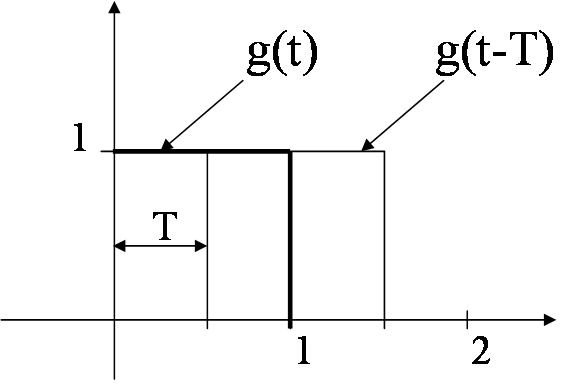
\includegraphics[width=7cm]{figprob4T3.png}
\end{center}

\vskip 0.2 cm
$Y(t) \in \{0, 1\}$, per tant \'es una v.a. discreta. 
\[
\begin{array}{ll}
P(Y(t)=y)& = 0 \text{ si } y \notin \{0, 1 \} 
\\ \\
P(Y(t)=1)& = P(g(t-T)=1)=P(0 < t-T < 1))=P(t-1 < T < t) = F_T(t)-F_T(t-1)=\\ \\        
         & = \begin{cases} 
             \text{si } t < 0 \qquad (\Rightarrow \,\, F_T(t)=F_T(t-1)=0) & 0-0=0 \\
             \text{si } 0 \leq t < 1 \qquad (\Rightarrow \,\, F_T(t)=t \, , \, F_T(t-1)=0) & t-0=t \\
             \text{si } 1 \leq t < 2 \qquad (\Rightarrow \,\, F_T(t)=1 \, , \, F_T(t-1)=t-1) & 1-(t-1)=2-t \\
             \text{si } t \geq 2 \qquad (\Rightarrow \,\, F_T(t)=F_T(t-1)=1) & 1-1=0 
             \end{cases}
\\ \\
P(Y(t)=0)& = 1-P(Y(t)=1)= \\ \\
         & = \begin{cases} 
             \text{si } t < 0 & 1-0=1 \\
             \text{si } 0 \leq t < 1 & 1-t \\
             \text{si } 1 \leq t < 2 & 1-(2-t)=t-1 \\
             \text{si } t \geq 2 & 1-0=1 
             \end{cases}
\end{array}
\]

\vskip 0.2 cm
\noindent
\textbf{b)}
\[
\mu_Y(t)=0 \cdot P(Y(t)=0) + 1 \cdot P(Y(t) = 1)=P(Y(t)=1)=\begin{cases} 
             \text{si } t < 0 & 0 \\
             \text{si } 0 \leq t < 1 & t \\
             \text{si } 1 \leq t < 2 & 2-t\\
             \text{si } t \geq 2 & 0 
             \end{cases}
\]

\newpage
\noindent
\textbf{c)} 

$C_Y(t_1, t_2)=R_Y(t_1, t_2)-\mu_Y(t_1) \cdot \mu_Y(t_2)$

\vskip 0.2 cm
\[
\begin{array}{ll}
R_Y(t_1, t_2)= & 0 \cdot 0 \cdot P(Y(t_1)=0, Y(t_2)=0) + 
0 \cdot 1 \cdot P(Y(t_1)=0, Y(t_2)=1) + \\ \\
               & + 1 \cdot 0 \cdot P(Y(t_1)=1, Y(t_2)=0) + 
1 \cdot 1 \cdot P(Y(t_1)=1, Y(t_2)=1) = P(Y(t_1)=1, Y(t_2)=1)
\end{array}
\]

\vskip 0.3 cm
\noindent
Cas $t_1=0.5$, $t_2=0.75$:

\vskip 0.2 cm
$P(Y(0.5)=1, Y(0.75)=1)=P(T < 0.5)=F_T(0.5)=0.5$

\vskip 0.2 cm
$\mu_Y(0.5)=0.5$

\vskip 0.2 cm
$\mu_Y(0.75)=0.75$


\vskip 0.2 cm
$C_Y(0.5, 0.75)=0.5- 0.5 \cdot 0.75 = 0.125$


\vskip 0.5 cm
\noindent
Cas $t_1=1.2$, $t_2=1.5$:


\vskip 0.2 cm
$P(Y(1.2)=1, Y(1.5)=1)=P(T > 0.5)=1-P(T \leq 0.5)=1-F_T(0.5)=1-0.5=0.5$

\vskip 0.2 cm
$\mu_Y(1.2)=2-1.2=0.8$

\vskip 0.2 cm
$\mu_Y(1.5)=2-1.5=0.5$


\vskip 0.2 cm
$C_Y(0.5, 0.75)=0.5- 0.8 \cdot 0.5 = 0.1$



\newpage

\vskip 0.5 cm
\noindent
\textbf{Problema 5.}
Sigui $Y(t)=g(t-T)$ el proc\'es del problema anterior per\`o amb
$T$ una v.a. exponencial de  par\`ametre $\lambda$.
\begin{enumerate}[a)]
\item Calculau la funci\'o de probabilitat de $Y(t)$.
\item Trobau la funci\'o $\mu_{Y}(t)$
\item Calculau $C_{Y}(0.2,1.2)$ y $C_Y(1.5, 1.5)$.
\end{enumerate}

\vskip 0.3 cm
\noindent
\textbf{Soluci\'o:}

\vskip 0.2 cm
\noindent
\textbf{a)} La seg\"uent figura mostra la forma de $g(t)$ i de $g(t-T)$,
on $T > 0$. A m\'es, com que $T \sim \mathrm{Exp}(\lambda)$,  
$F_T(t)=\begin{cases} 0 & \text{si } t \leq 0 \\ 1-e^{-\lambda t} & \text{si } t > 0  \end{cases}$

\vskip 0.2 cm
\begin{center}
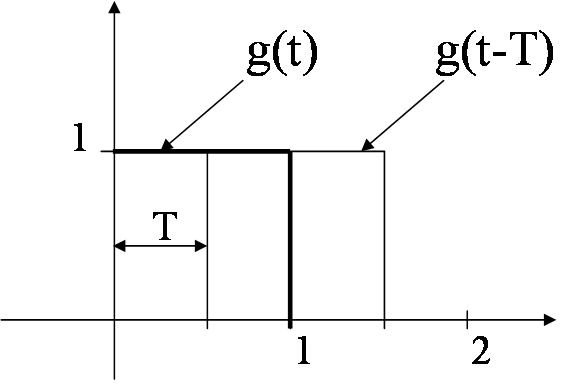
\includegraphics[width=7cm]{figprob4T3.png}
\end{center}

\vskip 0.2 cm
$Y(t) \in \{0, 1\}$, per tant \'es una v.a. discreta. 
\[
\begin{array}{ll}
P(Y(t)=y)& = 0 \text{ si } y \notin \{0, 1 \} 
\\ \\
P(Y(t)=1)& = P(g(t-T)=1)=P(0 < t-T < 1))=P(t-1 < T < t) = F_T(t)-F_T(t-1)=\\ \\        
         & = \begin{cases} 
\text{si } t \leq 0 \qquad (\Rightarrow \,\, F_T(t)=F_T(t-1)=0) & 0-0=0 \\
\text{si } 0 < t \leq 1 \qquad (\Rightarrow \,\, F_T(t)=1-e^{-\lambda t}\, , \, F_T(t-1)=0) & 
1-e^{-\lambda t}-0=1-e^{-\lambda t} \\
\text{si } t > 1 \qquad (\Rightarrow \,\, F_T(t)=1-e^{-\lambda t}\, , \, F_T(t-1)=1-e^{-\lambda (t-1)}) &
 e^{-\lambda t} (e^\lambda -1)
\end{cases}
\\ \\
P(Y(t)=0)& = 1-P(Y(t)=1)= \\ \\
         & = \begin{cases} 
             \text{si } t \leq 0 & 1-0=1 \\
             \text{si } 0 < t \leq 1 & 1-(1-e^{-\lambda t})=e^{-\lambda t} \\
             \text{si } t > 1 & 1-e^{-\lambda t} (e^\lambda -1) 
             \end{cases}
\end{array}
\]

\vskip 0.2 cm
\noindent
\textbf{b)}
\[
\mu_Y(t)=0 \cdot P(Y(t)=0) + 1 \cdot P(Y(t) = 1)=P(Y(t)=1)=\begin{cases} 
             \text{si } t \leq 0 & 0 \\
             \text{si } 0 < t \leq 1 & 1-e^{-\lambda t} \\
             \text{si } t > 1 & e^{-\lambda t} (e^\lambda -1)
             \end{cases}
\]


\vskip 0.2 cm
\noindent
\textbf{c)} 

$C_Y(t_1, t_2)=R_Y(t_1, t_2)-\mu_Y(t_1) \cdot \mu_Y(t_2)$

\vskip 0.2 cm
\[
\begin{array}{ll}
R_Y(t_1, t_2)= & 0 \cdot 0 \cdot P(Y(t_1)=0, Y(t_2)=0) + 
0 \cdot 1 \cdot P(Y(t_1)=0, Y(t_2)=1) + \\ \\
               & + 1 \cdot 0 \cdot P(Y(t_1)=1, Y(t_2)=0) + 
1 \cdot 1 \cdot P(Y(t_1)=1, Y(t_2)=1) = P(Y(t_1)=1, Y(t_2)=1)
\end{array}
\]

\vskip 0.3 cm
\noindent
Cas $t_1=0.2$, $t_2=1.2$:

\vskip 0.2 cm
$P(Y(0.2)=1, Y(1.2)=1)=P( (0 < T < 0.2) \cap (0.2 < T < 1.2))=P(\emptyset)=0$

\vskip 0.2 cm
$\mu_Y(0.2)=1-e^{-0.2 \lambda}$

\vskip 0.2 cm
$\mu_Y(1.2)=e^{-1.2 \lambda} (e^{\lambda}-1)$


\vskip 0.2 cm
$C_Y(0.2, 1.2)=0- (1-e^{-0.2 \lambda}) \cdot e^{-1.2 \lambda} (e^{\lambda}-1) = 
(e^{-0.2 \lambda}-1) e^{-1.2 \lambda} (e^{\lambda}-1)
$


\vskip 0.5 cm
\noindent
Cas $t_1=1.5$, $t_2=1.5$:


\vskip 0.2 cm
$P(Y(1.5)=1, Y(1.5)=1)=P(0.5 < T < 1.5)=F_T(1.5)-F_T(0.5)=(1-e^{-1.5 \lambda})-(1-e^{-0.5 \lambda})=$

$\qquad \qquad =e^{-0.5 \lambda}-e^{-1.5 \lambda}$

\vskip 0.2 cm
$\mu_Y(1.5)=e^{-1.5 \lambda} (e^{\lambda}-1)$


\vskip 0.2 cm
$C_Y(1.5, 1.5)=e^{-0.5 \lambda}-e^{-1.5 \lambda}- ( e^{-1.5 \lambda} (e^{\lambda}-1) )^2
$



\newpage

\noindent
\textbf{Problema 6.}  
Sigui $Z(t)=A t+B$ on $A$ i $B$ s\'on v.a. independents.

\begin{enumerate}[a)]
\item Calculau la funci\'o de densitat de $Z(t)$.
\item Trobau $\mu_{Z}(t)$ i $C_{Z}(t_{1},t_{2})$.
\end{enumerate}

\vskip 0.3 cm
\noindent
\textbf{Soluci\'o:}

\vskip 0.2 cm
\noindent
\textbf{b)} 

\[
\begin{array}{l}
\mu_Z(t)=E(Z(t))=E(At+B)=t E(A) + E(B) \\ \\
\begin{array}{ll}
R_Z(t_1, t_2) & = E(Z(t_1) \cdot Z(t_2))=E( (At_1+B) \cdot (At_2+B) )= \\ \\
 & = E(A^2 t_1 t_2 + AB (t_1+t_2) + B^2)= t_1 t_2 E(A^2) + (t_1+t_2) E(AB) + E(B^2)
\end{array}
\\ \\
\begin{array}{ll}
C_Z(t_1, t_2) &= R_Z(t_1, t_2) - \mu_Z(t_1) \mu_Z(t_2) = \\ \\
&= t_1 t_2 E(A^2) + (t_1+t_2) E(AB) + E(B^2) - (t_1 E(A) + E(B)) \cdot (t_2 E(A) + E(B)) = \\ \\
&= t_1 t_2 (E(A^2)-E(A)^2) + (t_1+t_2) (E(A) E(B) - E(A) E(B)) + (E(B^2)-E(B)^2) = \\ \\
&= t_1 t_2 \mathrm{Var}(A) + \mathrm{Var}(B)
\end{array}
\end{array}
\]

\noindent
On s'ha aplicat que $E(AB)=E(A)E(B)$, ja que les v.a. s\'on independents.

\newpage

\noindent
\textbf{Problema 7.}  
Trobau una expressi\'o de $E((X(t_{2})-X(t_{1}))^2)$ en termes
de la funci\'o d'autocorrelaci\'o.


\vskip 0.3 cm
\noindent
\textbf{Soluci\'o:}

\[
\begin{array}{ll}
E((X(t_{2})-X(t_{1}))^2) & =E(X(t_2)^2 - 2 X(t_1) X(t_2) + x(t_1)^2)=
E(X(t_2)^2) - 2 E(X(t_1) X(t_2)) + E(x(t_1)^2)= \\ \\
 & = R_X(t_1, t_1)+R_X(t_2, t_2)-2 R_X(t_1, t_2)
\end{array}
\]


\vskip 1.5 cm
\noindent
\textbf{Problema 8.}  
 ?`Un proc\'es ortogonal  \'es incorrelat? ?`Un proc\'es incorrelat
\'es ortogonal?

\vskip 0.3 cm
\noindent
\textbf{Soluci\'o:}

\vskip 0.2 cm
\noindent
Recordem que:

$X(t)$ i $Y(t)$ ortogonals $\Longleftrightarrow$ $R_{XY}(t_1, t_2) = 0 \qquad \forall t_1, t_2$

$X(t)$ i $Y(t)$ incorrelats $\Longleftrightarrow$ $C_{XY}(t_1, t_2) = 0 \qquad \forall t_1, t_2$

\vskip 0.2 cm
\noindent
ortogonal $\Longleftrightarrow$ incorrelat? NO

si $R_{XY}(t_1, t_2) = 0$, llavors 
$C_{XY}(t_1, t_2) =R_{XY}(t_1, t_2)-\mu_X(t_1) \cdot \mu_Y(t_2)=\mu_X(t_1) \cdot \mu_Y(t_2) \neq 0 \,$
 (en general)

 
\vskip 0.2 cm
\noindent
incorrelat $\Longleftrightarrow$ ortogonal? NO

si $C_{XY}(t_1, t_2) = 0$, llavors 
$R_{XY}(t_1, t_2) =C_{XY}(t_1, t_2)+\mu_X(t_1) \cdot \mu_Y(t_2)=\mu_X(t_1) \cdot \mu_Y(t_2) \neq 0 \,$
 (en general)

\newpage

\noindent
\textbf{Problema 13.}  
Sigui $M(n)$ un proc\'es discret definit com la seq\"{u}\`encia de
les mitjanes d'una successi\'o de v.a. $X_i$ iid:

$$M(n)=\frac{X_{1}+\cdots +X_{n}}{n}$$
Trobau la mitjana,la vari\`ancia i l'autocovari\`ancia de $M(n)$.

\vskip 0.3 cm
\noindent
\textbf{Soluci\'o:}

\vskip 0.2 cm
\noindent

\[
E(M(n))=E \left( \frac{X_{1}+\cdots +X_{n}}{n} \right)=\frac{1}{n} \cdot  E(X_1+\cdots+X_n)=\text{(i.i.d.)}=
\frac{1}{n} \cdot n \cdot E(X)=E(X)
\]

\[
\mathrm{Var}(M(n))=\mathrm{Var} \left( \frac{X_{1}+\cdots +X_{n}}{n} \right)=\frac{1}{n^2} \cdot  \mathrm{Var}(X_1+\cdots+X_n)=\text{(i.i.d.)}=
\frac{1}{n^2} \cdot n \cdot \mathrm{Var}(X)=\frac{\mathrm{Var}(X)}{n}
\]

\vskip 0.2 cm
\noindent
Calculam l'autocorrelaci\'o i l'autocovari\`ancia en el cas $k \geq n$:

\[
\begin{array}{rl}
R_M(n, k)& =E(M(n) \cdot M(k))=E \left( \frac{X_{1}+\cdots +X_{n}}{n} \cdot \frac{X_{1}+\cdots +X_{k}}{k} \right)=
\\ \\
& = \frac{1}{nk} E(X_1 X_1 + X_1 X_2 + \cdots + X_n X_k) = 
\frac{1}{nk} \cdot \left[ E(X_1 X_1) + E(X_1 X_2) + \cdots + E(X_n X_k) \right]=\\ \\
& = \frac{1}{nk} \sum_{i=1}^n \sum_{j=1}^k E(X_i X_j) = 
\frac{1}{nk} \left[ \sum_{i=1}^n \sum_{j=1, j \neq i}^k E(X_i X_j) + \sum_{i=1}^n E(X_i^2) \right] = \\ \\
& = (E(X_i X_j)=E(X_i) \cdot E(X_j) \text{ si $i \neq j$, ja que $X_i$ i $X_j$ s\'on independents})  = \\ \\
&= \frac{1}{nk} \left[ \sum_{i=1}^n \sum_{j=1, j \neq i}^k E(X) \cdot E(X) + \sum_{i=1}^n E(X^2) \right] = \\ \\
& = \frac{1}{nk} \left[ (nk-n) E(X)^2 + n (\mathrm{Var}(X)+E(X)^2) \right]=E(X)^2 + \frac{\mathrm{Var}(X)}{k}
\end{array}
\]

\[
\begin{array}{rl}
C_M(n, k) & =R_M(n, k)-E(M(n)) \cdot E(M(k))=R_M(n, k)-E(X)^2=E(X)^2 + \frac{\mathrm{Var}(X)}{k}-E(X)^2= \\ \\
& =\frac{\mathrm{Var}(X)}{k}=\mathrm{Var}(M(k))=C_M(k, k)
\end{array}
\]

\newpage


\noindent
\textbf{Problema 14.}  
Suposem que una secret\`aria rep cridades  que  arriben
d'acord amb un proc\'es de Poisson amb un ritme de 10 cridades per
hora. Quina \'es la probabilitat  que cap cridada es quedi sense
resposta si la secret\`aria surt de l'oficina els primers 15 i els
darrers 15 minuts d'una hora?

\vskip 0.3 cm
\noindent
\textbf{Soluci\'o:}

\vskip 0.2 cm
\noindent
Definim el proc\'es $X(t)=$ \textit{nombre de cridades en el per\'iode} $(0, t)$ (temps en minuts).
Per l'enunciat sabem que $X(t) \sim \mathrm{Po}(\lambda t)$, amb $\lambda=10$.

Per a que cap cridada quedi sense
resposta si la secret\`aria surt de l'oficina els primers 15 i els
darrers 15 minuts d'una hora ha de passar que no es rebi cap 
cridada durant els primers 15 minuts ni durant els darrers 15 minuts:
\[
P(\text{cap cridada perduda})=P(\text{cap cridada primers 15 min.} \cap \text{cap cridada darrers 15 min.})
\]
Si les cridades s\'on independents entre s\'i podem escriure
\[
P(\text{cap cridada perduda})=P(\text{cap cridada primers 15 min.}) \cdot P(\text{cap cridada darrers 15 min.})
\]

D'altra banda:
\[
P(\text{cap cridada primers 15 min.})=P(\text{0 cridades en per\'iode } (0, \frac{1}{4}))=
P(X(\frac{1}{4})=0)
\]

Com que $X(\frac{1}{4}) \sim \mathrm{Po}(\lambda \frac{1}{4})=\mathrm{Po}(2.5)$, llavors 
$P(X(\frac{1}{4})=0)=\frac{2.5^0}{0!} e^{-2.5}=0.082$.

\vskip 0.3 cm
Tenim a m\'es que el nombre de cridades en els darrers 15 minuts \'es igual al nombre de cridades
rebudes fins al minut 60 (en el per\'iode de 0 a 1 hora) menys el nombre de cridades rebudes fins 
al minut 45 (en el per\'iode de 0 a $\frac{3}{4}$ d'hora). Per tant:
\[
P(\text{cap cridada darrers 15 min.})=P( X(1)-X(\frac{3}{4}) = 0)
\]

D'altra banda, es pot demostrar que si $A \sim \mathrm{Po}(\lambda)$ i $B \sim \mathrm{Po}(\mu)$
i $A \geq B$, llavors $A-B \sim \mathrm{Po}(\lambda-\mu)$. Aplicant aquesta propietat al nostre 
problema tenim que $X(1) \sim \mathrm{Po}(10)$, $X(\frac{3}{4}) \sim \mathrm{Po}(7.5)$, per tant
$X(1)-X(\frac{3}{4}) \sim \mathrm{Po}(10-7.5)=\mathrm{Po}(2.5)$. De manera que:
\[
P( X(1)-X(\frac{3}{4}) = 0) = \frac{2.5^0}{0!} e^{-2.5}=0.082
\]


Per tant el resultat final \'es:
\[
P(\text{cap cridada perduda})=0.082 \cdot 0.082=0.006724
\]


\newpage

\noindent
\textbf{Problema 14.}
Suposem que una secret\`aria rep cridades  que  arriben
d'acord amb un proc\'es de Poisson amb un ritme de 10 cridades per
hora. Quina \'es la probabilitat  que cap cridada es quedi sense
resposta si la secret\`aria surt de l'oficina els primers 15 i els
darrers 15 minuts d'una hora?

\vskip 0.3 cm
\noindent
\textbf{Soluci\'o:}

\vskip 0.2 cm
\noindent
L'enunciat ens diu que es tracta d'un proc\'es de Poisson, per tant,
si definim $X(t)$ com el \textit{nombre de cridades en el periode $(0, t)$}
tenim que $X(t) \sim \mathrm{Po}(\lambda t)$.

\[
\begin{array}{l}
P(\text{cap cridada sense resposta})=P( \{ X(15 \text{min.})=0 \} \cap \{ X(1 \text{h.})-X(45 \text{min.}) = 0 \} )= \\ \\
=P( \{ X(1/4) = 0 \} \cap \{ X(1)-X(3/4) = 0 \} )=\text{cridades independents}=P(X(1/4) = 0) \cdot P( X(1)-X(3/4) = 0 )
\end{array}
\]

\vskip 0.3 cm
\noindent
D'altra banda, si $X(t) \sim \mathrm{Po}(\lambda t)$ es verifica que $X(t_2)-X(t_1) \sim \mathrm{Po}(\lambda(t_2-t_1)) \sim X(t_2-t_1)$,
sempre que $t_2 > t_1$. Per tant:

\[
\begin{array}{ll}
P(X(1/4) = 0) \cdot P( X(1)-X(3/4) = 0 )&=P(X(1/4) = 0) \cdot P( X(1-3/4) = 0 )=P(X(1/4) = 0) \cdot P( X(1/4) = 0 )= \\ \\
&= \left( \frac{(10/4)^0}{0!} e^{-10/4} \right)^2 = e^{-5}=0.006738
\end{array}
\]


\vskip 2cm 
\noindent
\textbf{Problema 16.}
Un impuls de renou ocorr en una l\'{\i}nia telef\`onica d'acord amb
un proc\'es Poisson de par\`ametre $\lambda$ per segon.

\begin{enumerate}[a)]
\item Trobau la probabilitat  que no ocorri cap impuls
en  el transcurs d'un missatge de $t$ segons.
\item Suposem que el missatge est\`a codificat i que si s'ha
produ\"{\i}t un impuls podem corregir el missatge. Quina \'es la
probabilitat  que un missatge de $t$ segons estigui lliure
d'errors o es pugui corregir?
\end{enumerate}

\vskip 0.3 cm
\noindent
\textbf{Soluci\'o:}

\vskip 0.2 cm
\noindent
Definim $N(t)$ com el \textit{nombre d'impulsos de renou en $t$ segons}. Per l'enunciat
$N(t) \sim \mathrm{Po}(\lambda t)$.

\vskip 0.2 cm
\noindent
\textbf{a)} 
\[
P(N(t) = 0)=\frac{ (\lambda t)^0 }{0!} e^{-\lambda t}=e^{-\lambda t}
\]

\vskip 0.2 cm
\noindent
\textbf{b)}

\[
P(N(t) \leq 1)=P(N(t)=0)+P(N(t)=1)=\frac{ (\lambda t)^0 }{0!} e^{-\lambda t} + \frac{ (\lambda t)^1 }{1!} e^{-\lambda t} = 
(1+\lambda t) e^{-\lambda t} 
\]

 



\newpage
\noindent
\textbf{Problema 15.}
Els clients arriben  a una m\`aquina de refrescs segons un
proc\'es Poisson de mitjana $\lambda$. Suposem que cada vegada que
un client deposita una moneda, la m\`aquina dispensa un refresc amb
probabilitat $p$. Trobau la funci\'o de probabilitat del nombre de
begudes dispensades en un temps $t$. (Nota: s'ha de suposar que la
m\`aquina cont\'e un nombre ilimitat  de refrecs).  

\vskip 0.3 cm
\noindent
\textbf{Soluci\'o:}

\vskip 0.2 cm
\noindent
Definim:

$N(t)$: \textit{nombre de begudes dispensades en un temps $t$}

$C(t)$: \textit{nombre de clients que arriben a la m\`aquina de begudes en un temps $t$}, per l'enunciat
$C(t) \sim \mathrm{Po}(\lambda t)$.

\vskip 0.3 cm
Podem calcular la probabilitat de $N(t)$ aplicant la f\'ormula de
la probabilitat total:

\[
\begin{array}{rl}
P(N(t) = k) & =P(N(t)=k | C(t)=k) \cdot P(C(t)=k) + P(N(t)=k | C(t)=k+1) \cdot P(C(t)=k+1) + \cdots=\\ \\
&= \sum_{n=k}^\infty P(N(t)=k | C(t)=n) \cdot P(C(t)=n)
\end{array}
\]

D'altra banda, si definim $Y$ com $Y=N(t)|_{C(t)=n}$, llavors $Y$ compta el nombre de begudes
dispensades amb \`exit d'un total de $n$ intents. Per tant $Y \sim B(n, p)$ i
$P(N(t)=k | C(t)=k)=P(Y=k)=\binom{n}{k} p^k (1-p)^{n-k}$. De manera que:

\[
\begin{array}{rl}
P(N(t) = k) & = \sum_{n=k}^\infty \binom{n}{k} p^k (1-p)^{n-k} \frac{(\lambda t)^n}{n!} e^{-\lambda t} = \\ \\
& = e^{-\lambda t} \sum_{n=k}^\infty  \frac{n!}{(n-k)! k!} (\frac{p}{1-p})^k (1-p)^n \frac{(\lambda t)^n}{n!} =
 \\ \\
& = e^{-\lambda t} \frac{1}{k!} (\frac{p}{1-p})^k \sum_{n=k}^\infty \frac{ ((1-p)\lambda t)^n}{(n-k)!}
\end{array}
\]

En el sumatori feim el canvi de variable $m=n-k$, de manera que quan $n=k$, $m=0$ i quan 
$n=\infty$, $m=\infty$:

\[
\begin{array}{rl}
P(N(t) = k)& = e^{-\lambda t} \frac{1}{k!} (\frac{p}{1-p})^k \sum_{m=0}^\infty \frac{ ((1-p)\lambda t)^{m+k}}{m!}
= \\ \\ & 
e^{-\lambda t} \frac{1}{k!} (\frac{p}{1-p})^k (1-p)^k (\lambda t)^k \sum_{m=0}^\infty 
\frac{((1-p)\lambda t)^m}{m!}
\end{array}
\]

Aplicant la igualtat seg\"uent (obtinguda a partir del polinomi de Taylor): 
$e^x=\sum_{m=0}^\infty \frac{x^m}{m!}$, tenim que

\[
P(N(t) = k)= e^{-\lambda t} \frac{1}{k!} p^k (\lambda t)^k  e^{((1-p)\lambda t)}=
\frac{(\lambda t p)^k}{k!} e^{-\lambda t p}
\]

Aquesta expressi\'o correspon a la funci\'o de probabilitat de una v.a. de 
Poisson amb par\`ametre $\lambda t p$, per tant: 
\[
N(t) \sim \mathrm{Po}(\lambda t p)
\]


\newpage

\noindent
\textbf{Problema 17.}
Els missatges arriben a un ordinador desde dues l\'{\i}nies
telef\`oniques segons dos processos de Poisson independents i amb
ritmes $\lambda_{1}$ i $\lambda_{2}$ respectivament.
\begin{enumerate}[a)]
    \item Trobau la probabilitat  que un missatge arribi primer per la
    linea $1$.
    \item  Trobau la funci\'o de densitat del temps que tarda un
    missatge en arribar per alguna de les l\'inies.
    \item Trobau la probabilitat de $N(t)$ el nombre total de
    missatges
    que arriben a l'ordinador en un interval de longitud $t$.
    \item  Generalitzau el resultat anterior quan es junten $k$
    l\'{\i}nies telef\`oniques independents Poisson amb par\`ametres
$\lambda_{1},\ldots,\lambda_{k}$ y
$N(t)=N_{1}(t)+\ldots+N_{k}(t)$.
\end{enumerate}

\vskip 0.3 cm
\noindent
\textbf{Soluci\'o:}

\vskip 0.2 cm
\noindent
\textbf{a)} Definim

$N_1(t)$: \textit{nombre de missatges enviats per la l\'inia 1 en el per\'iode $(0, t)$}

$N_2(t)$: \textit{nombre de missatges enviats per la l\'inia 2 en el per\'iode $(0, t)$}

$T_1$: \textit{temps que tarda en arribar un missatge per la l\'inia 1}

$T_2$: \textit{temps que tarda en arribar un missatge per la l\'inia 2}

\vskip 0.3 cm
Ens demanen calcular $P(T_1 < T_2)$:

\[
P(T_1 < T_2)=P(T_1 - T_2 < 0)=\iint_A f_{T_1 T_2}(t_1, t_2) \, dt_1 \, dt_2
\]

\noindent
on $A$ \'es el conjunt de valors $(t_1, t_2)$ tals que $t_1-t_2 < 0$ i $f_{T_1 T_2}$ \'es
la funci\'o de densitat conjunta de $T_1$ i $T_2$ (consideram que s\'on v.a. cont\'inues). 
Com les dues l\'inies s\'on independents
llavors $f_{T_1 T_2}(t_1, t_2)=f_{T_1}(t_1) \cdot f_{T_2}(t_2)$.

Per a calcular les funcions de densitat 
de $T_1$ i $T_2$ comen\c{c}am calculant les funcions de distribuci\'o:

\[
\begin{array}{rl}
F_{T_1}(t) & =P(T_1 \leq t)=\text{(el missatge arriba abans de $t$ segons)}=
\text{(en $t$ segons s'ha rebut al menys 1 missatge)}= \\ \\
& = P(N_1(t) \geq 1) = 1- P(N_1(t) \leq  0)=1- P(N_1(t)= 0)=
1- \frac{(\lambda_1 t)^0}{0!} e^{-\lambda_1 t} =1-e^{-\lambda_1 t}
\end{array} 
\]

\noindent
Aquest resultat \'es v\`alid quan $t \geq 0$, en cas contrari $F_{T_1}(t)=0$. En resum:
\[
F_{T_1}(t)=\begin{cases} 1-e^{-\lambda_1 t} & \text{si } t\geq 0 \\ 0 & \text{si } t < 0 \end{cases}
\]

Aquesta funci\'o de distribuci\'o correspon a una v.a. exponencial amb par\`ametre $\lambda_1$, per tant
$T_1 \sim \mathrm{Exp}(\lambda_1)$. Raonant de manera similar trobariem que $T_2 \sim \mathrm{Exp}(\lambda_2)$.
Per tant:

\[
f_{T_1 T_2}(t_1, t_2)=f_{T_1}(t_1) \cdot f_{T_2}(t_2)=\begin{cases}
\lambda_1 \lambda_2 e^{-\lambda_1 t_1 - \lambda_2 t_2} & \text{si } t_1 > 0 \text{ i } t_2 > 0 \\ \\
0 & \text{altrament} \end{cases}
\]

Ara ja podem calcular la probabilitat que ens demanen. La regi\'o d'integraci\'o $A$ t\'e la forma
dun triangle limitat per l'eix $t_2$ i la recta $t_1-t_2=0$. 

\[
P(T_1 < T_2)=\int_0^\infty \int_{t_1}^\infty \lambda_1 \lambda_2 
e^{-\lambda_1 t_1 - \lambda_2 t_2} \, d_{t_2} \, d_{t_1}= \cdots =\frac{\lambda_1}{\lambda_1 + \lambda_2}
\]

\vskip 0.2 cm
\noindent
\textbf{b)} Definim $T$: \textit{temps que tarda en arribar un missatge per alguna de les l\'inies}.
Calculam primer la funci\'o de distribuci\'o de $T$:

\[
\begin{array}{rl}
P(T \leq t) & =P(T_1 \leq t \, \cup \, T_2 \leq t)=P(T_1 \leq t) + P(T_2 \leq t) - 
P(T_1 \leq t \, \cap \, T_2 \leq t)=
\text{($T_1$ i $T_2$ independents)}= \\ \\
& = P(T_1 \leq t) + P(T_2 \leq t) - P(T_1 \leq t) \cdot P(T_2 \leq t)=
(1-e^{-\lambda_1 t}) + (1-e^{-\lambda_2 t}) - (1-e^{-\lambda_1 t}) \cdot (1-e^{-\lambda_2 t})=\\ \\
&= \cdots = 1-e^{(\lambda_1+\lambda_2)t}
\end{array}
\]

\noindent
Aquest resultat \'es v\`alid si $t \geq 0$, en cas contrari $P(T \leq t)=0$.
El resultat obtengut correspon a la funci\'o de distribuci\'o d'una v.a. exponencial amb 
par\`ametre $\lambda_1+\lambda_2$. Per tant: 
\[
T \sim \mathrm{Exp}(\lambda_1+\lambda_2)
\]

\vskip 0.2 cm
\noindent
\textbf{c)} Definim $N(t)$:\textit{nombre total de missatges en el per\'iode $(0, t)$}.
Tenim que $N(t)=N_1(t)+N_2(t)$.

\[
\begin{array}{rl}
P(N(t)=k) & = P(N_1(t)+N_2(t)=k)=\text{(f\'ormula de la prob. total)}= \\ \\
&= P(N_1(t)+N_2(t)=k |_{N_1(t)=0}) \cdot P(N_1(t)=0) + P(N_1(t)+N_2(t)=k |_{N_1(t)=1}) \cdot P(N_1(t)=1)+\cdots 
+ \\ \\
& \quad + P(N_1(t)+N_2(t)=k |_{N_1(t)=k}) \cdot P(N_1(t)=k)= \\ \\
&= \sum_{i=0}^{k} P(N_1(t)+N_2(t)=k |_{N_1(t)=i}) \cdot P(N_1(t)=i) = \\ \\
& = \sum_{i=0}^{k} P(N_2(t)=k-i) \cdot P(N_1(t)=i) = 
\sum_{i=0}^{k} \frac{(\lambda_2 t)^{k-i}}{(k-i)!} e^{-\lambda_2 t} 
\frac{(\lambda_1 t)^{i}}{(i)!} e^{-\lambda_1 t} = \\ \\
& = e^{-(\lambda_1+\lambda_2)t} \sum_{i=0}^{k} \frac{1}{(k-i)! i!} (\lambda_2 t)^{k-i} (\lambda_1 t)^{i} = \\ \\
& = \frac{1}{k!} e^{-(\lambda_1+\lambda_2)t} \sum_{i=0}^{k} \binom{k}{i} (\lambda_1 t)^{i} (\lambda_2 t)^{k-i}
= \\ \\
& =\text{(aplicant la f\'ormula del binomi de Newton)}=\\ \\
& = \frac{1}{k!} e^{-(\lambda_1+\lambda_2)t} ((\lambda_1+\lambda_2)t)^k=
 \frac{ ((\lambda_1+\lambda_2)t)^k }{k!} e^{-(\lambda_1+\lambda_2)t}
\end{array}
\]

Aquesta funci\'o de probabilitat correspon a una v.a. de Poisson de par\`ametre $\lambda_1+\lambda_2$.
Per tant: 
\[
N(t) \sim \mathrm{Po}(\lambda_1+\lambda_2)
\]

\vskip 0.2 cm
\noindent
\textbf{d)} En aquest cas $N(t)=N_1(t)+N_2(t)+\cdots+N_k(t)$.
Raonant de manera similar a l'apartat anterior i agrupant les variables de dos en dos
de manera successiva arribarem a:
\[
N(t) \sim \mathrm{Po}(\lambda_1+\lambda_2+\cdots+\lambda_k)
\]

\newpage 
\noindent
\textbf{Exemple 6.}
Calculau $C_{XY}(t_1, t_2)$ per als processos $X(t)=\cos(\omega t + \Theta)$
i $Y(t)=\sin(\omega t + \Theta)$, on $\Theta \sim {\cal U}(-\pi, \pi)$.

\vskip 0.3 cm
\noindent
\textbf{Soluci\'o:}

\noindent
La funci\'o de densitat de ${\Theta}$ \'es

\[
f_{\Theta}(\theta)=\begin{cases} \frac{1}{2\pi} & \text{si } -\pi \leq \theta \leq \pi \\ \\
0 & \text{altrament} \end{cases}
\]

\noindent
Per tant:

\[
\begin{array}{ll}
\mu_X(t)& =E(X(t))=E(\cos(\omega t + \Theta))=\int_{\R} \cos(\omega t + \theta) f_{\Theta}(\theta) \, d\theta = \\ \\
& = \frac{1}{2\pi} \int_{-\pi}^{\pi} \cos(\omega t + \theta) \, d\theta = 0 \\ \\

& \text{(S'ha aplicat la propietat de que la integral d'un periode d'una funci\'o sinuso\"idal \'es 0)} \\ \\

\\

\mu_Y(t)& =E(Y(t))=E(\sin(\omega t + \Theta))=\int_{\R} \sin(\omega t + \theta) f_{\Theta}(\theta) \, d\theta = \\ \\
& = \frac{1}{2\pi} \int_{-\pi}^{\pi} \sin(\omega t + \theta) \, d\theta = 0 \\ \\ \\

C_{XY}(t_1, t_2) &= R_{XY}(t_1, t_2) - \mu_X(t_1) \mu_Y(t_2) = R_{XY}(t_1, t_2) - 0 = E(X(t_1) Y(t_2)) = \\ \\
&= E( \cos(\omega t_1 + \Theta) \sin(\omega t_2 + \Theta) ) =
 \frac{1}{2\pi} \int_{-\pi}^{\pi}  \cos(\omega t_1 + \theta) \sin(\omega t_2 + \theta) \, d\theta = \\ \\
&=\frac{1}{2\pi} \int_{-\pi}^{\pi}  \left( \frac{1}{2} \sin(\omega(t_1+t_2)+2\theta) - \frac{1}{2} \sin(\omega(t_1-t_2)) \right) \, d\theta= \\ \\
&= \frac{1}{2\pi} \int_{-\pi}^{\pi} \frac{1}{2} \sin(\omega(t_1+t_2)+2\theta) \, d\theta - 
\frac{1}{2\pi} \int_{-\pi}^{\pi} \frac{1}{2} \sin(\omega(t_1-t_2)) \, d\theta = \\ \\
&= 0 - \frac{1}{2} \sin(\omega(t_1-t_2)) \frac{1}{2\pi} \int_{-\pi}^{\pi}  d\theta = - \frac{1}{2} \sin(\omega(t_1-t_2)) \\ \\
& \text{(S'ha aplicat que $\cos A \cdot \sin B = \frac{1}{2} \sin(A+B) - \frac{1}{2} \sin (A-B) $ )}
\end{array}
\]


\end{document}
